\renewcommand{\theequation}{\theenumi}
%\renewcommand{\thefigure}{\theenumi}\
\setcounter{figure}{0}

\begin{enumerate}[label=\arabic*.,ref=\thesubsubsection.\theenumi]
\numberwithin{equation}{enumi}
\numberwithin{figure}{enumi}
%
\item Let 
%
\begin{align}
y &= 3x + 1
\\
\implies \myvec{3 & -1}\vec{x} &= -1
\label{eq:3.7.1.1}
\end{align}
%
For $x = \frac{1}{3}$ to be a zero, 
%
\begin{align}
\vec{x} = \myvec{\frac{1}{3} \\ 0}
\end{align}
%
should satisfy \eqref{eq:3.7.1.1}.

\begin{align}
\because \myvec{3 & -1} \myvec{\frac{1}{3} \\ 0} = 1
\ne -1,
\end{align}
%
$\vec{x}=\frac{1}{3}$ is not a zero. This is verified in Fig. \ref{fig:3.7.1_line1}.
%
\renewcommand{\thefigure}{\theenumi.\arabic{figure}}
\begin{figure}[!ht]
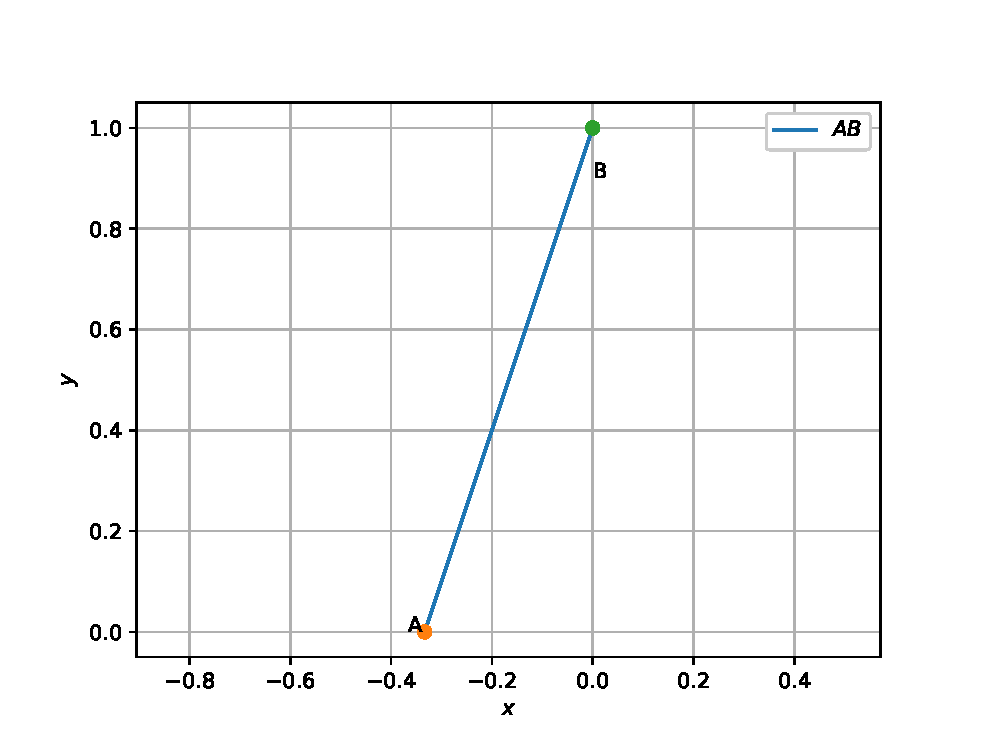
\includegraphics[width=\columnwidth]{./solutions/1/figs/line/line1.eps}
\caption{}
\label{fig:3.7.1_line1}
\end{figure}

\item Let 
%
\begin{align}
y &= 5x -\pi
\\
\implies \myvec{5 & -1}\vec{x} &= \pi
\end{align}
%
%
\begin{align}
\myvec{5 & -1}\myvec{\frac{4}{5}\\0} = 4 \ne \pi
\end{align}
%
Hence $\vec{x}=\frac{4}{5}$ is not a zero. This is verified in Fig. \ref{fig:3.7.1_line2}.
%
\begin{figure}[!ht]
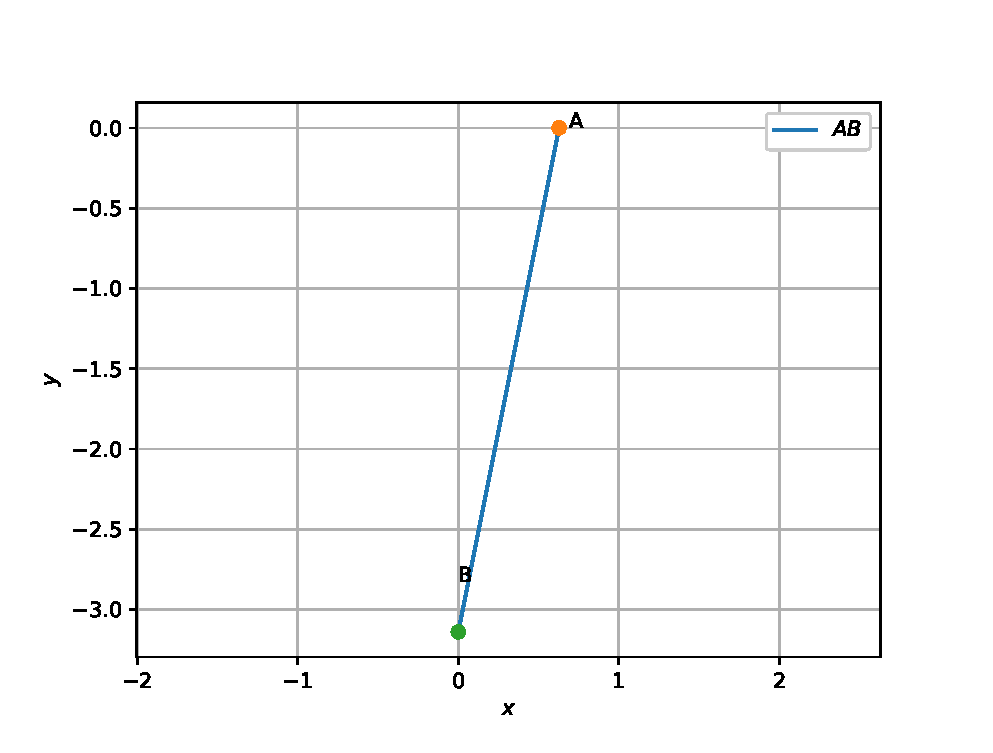
\includegraphics[width=\columnwidth]{./solutions/1/figs/line/line2.eps}
\caption{}
\label{fig:3.7.1_line2}
\end{figure}
\item Let 
%
\begin{align}
y &= 5lx + m
\\
\implies \myvec{5l & -1}\vec{x} &= -m
\end{align}
%
Thus, 
%
\begin{align}
 \myvec{5l & -1}\myvec{-\frac{m}{l}\\0} &= -5m \ne -m
\end{align}
%
Hence $\vec{x}=-\frac{m}{l}$ is not a zero. This is verified in Fig. \ref{fig:3.7.1_line3}.
%
\begin{figure}[!ht]
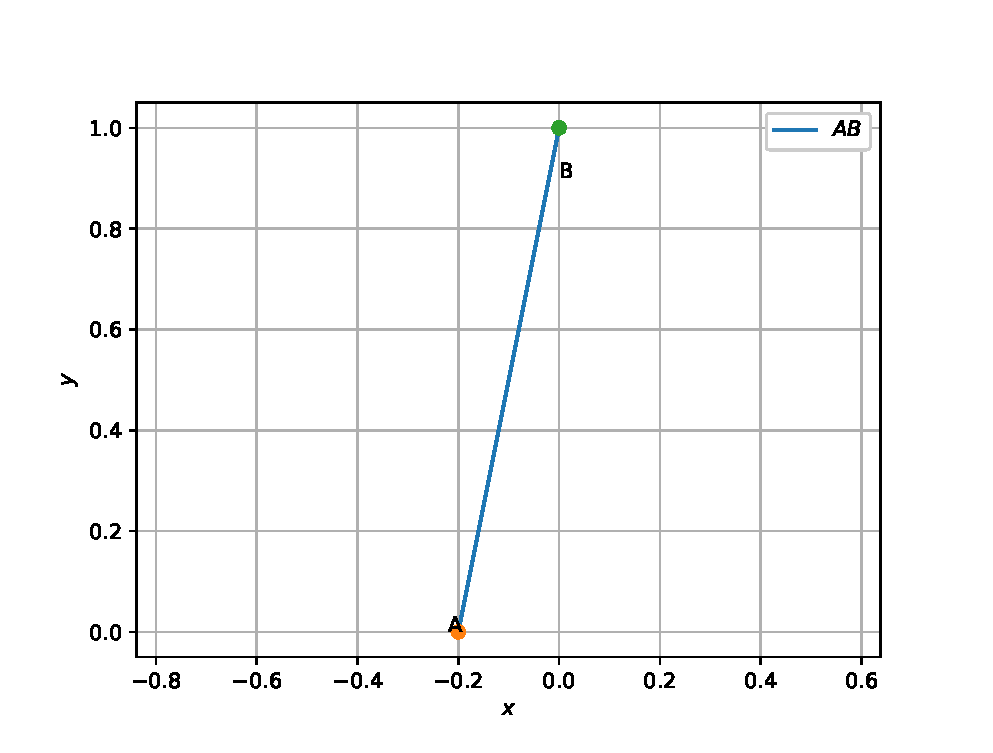
\includegraphics[width=\columnwidth]{./solutions/1/figs/line/line3.eps}
\caption{}
\label{fig:3.7.1_line3}
\end{figure}
\item Let 
%
\begin{align}
y &= 2x + 1
\\
\implies \myvec{2 & -1}\vec{x} &= -1
\end{align}
%
Thus, 
%
\begin{align}
\myvec{2 & -1}\myvec{\frac{1}{2}\\0} = 2 \ne -1
\end{align}
%
Hence $\vec{x}=\frac{1}{2}$ is not a zero. This is verified in Fig. \ref{fig:3.7.1_line4}.
%
\begin{figure}[!ht]
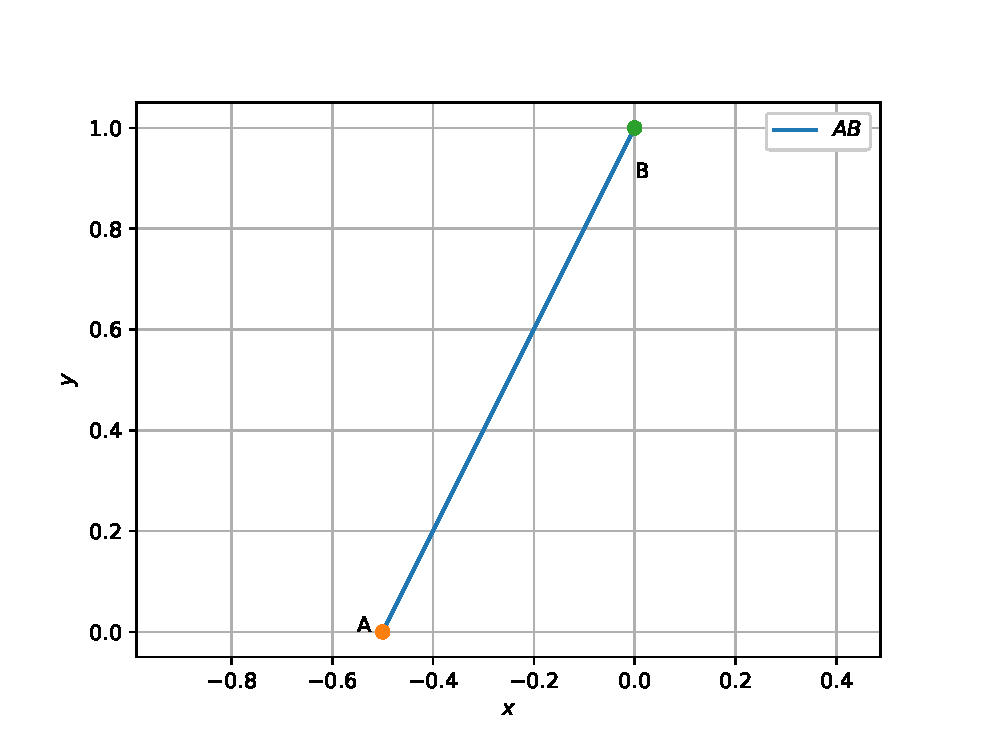
\includegraphics[width=\columnwidth]{./solutions/1/figs/line/line4.eps}
\caption{}
\label{fig:3.7.1_line4}
\end{figure}
\renewcommand{\thefigure}{\theenumi}
\end{enumerate}
